\chapter{Localisation using Android}
\label{chap:and-loc}

\section*{Introduction}
The localisation of the mobile device is a key system service of Android.
Many applications use this service, as a feature of the application.
It allows, for example, to show directly the part of the map where the user is on Google Maps, to display advertisements for nearby shops, to automatically select the relevant area for the weather forecast, to give statistical information regarding the using of an application in a particular region.\\

The details of the localisation methods used by the Android system are often unknown or unclear.
There exists several techniques to locate a device: using the GPS chip usually present in smartphones or using connection information (cell phone tower or wireless access points).
This chapter explains how these techniques work and why they are subject to privacy concerns.\\

Several facts about the management of the localisation have been used in the official declarations or documentations.
To verify these assumptions, several experiments have been carried out using an Android 2.3 smartphone.
These experiments allow us to have a better understanding of the localisation system that mostly works as a black box.


\section{GPS}
\label{sec:loc-gps}

% Today almost every smartphone have an embedded GPS chip.
% It is a very accurate way to locate the user.

\subsection{GPS signal}

The GPS, for Global Positioning System, is a technology based on satellite trilateration.
GPS satellites are navigating around the Earth in a way to maximise the number of visible satellites anywhere at any time.
There is currently 31 working satellites in orbit~\cite{pocketgpsworld}.
The location-aware device is equipped with a GPS receiver chip.
This receiver retrieves broadcasted messages from the reachable satellites.
The messages contain :

\begin{itemize}
\item the time the message was transmitted
\item precise orbital information (the ephemeris)
\item the general system health and rough orbits of all GPS satellites (the almanac)
\end{itemize}

Trilateration is used based on the received messages as shown in Figure \ref{fig:gps-earth}.
If, theoretically, three satellites are enough, at least four are required to avoid clock synchronisation errors (at the speed of light, even a small clock error can lead to huge distance gap).\\

% TODO changer image pour noir & blanc
\begin{figure}[h]
  \centering
  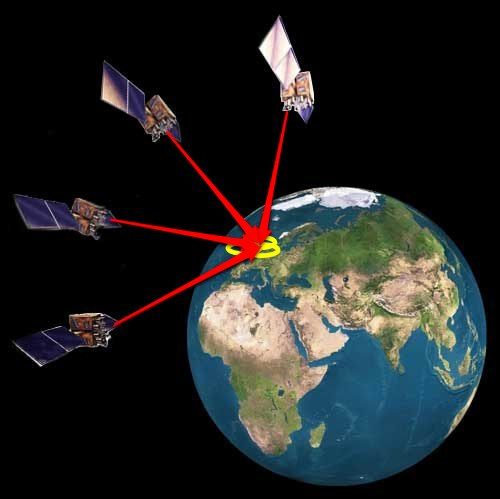
\includegraphics[width=6cm]{images/gps.jpg}
  \caption{Signals from multiple satellites are required to calculate a position\newline Copyright PocketGPSWorld.com}
  \label{fig:gps-earth}
\end{figure}


The accuracy of this method depends on the surrounding of the user.
In clear sight, the GPS is accurate to a few meters but it will degrade if the receiver is surrounded by high buildings or inside a dense forest.\\

The time to first fix (TTFF) depends on the state of the GPS.
In a cold start scenario\footnote{Device is in factory state or the GPS data are not relevant (several months old or inaccurate)}, the GPS needs to retrieve the full almanac.
This is done in at least 12.5 minutes~\cite{gpsuser}.
To improve the TTFF, embedded GPS often uses assisted-GPS technology (aGPS) by acquiring almanac and ephemeris data over a fast network connection when available.

\subsection{Degradation}

The GPS system was invented by the U.S. Department of Defence as a military project.
As the technology became available to civilians, it was intentionally degraded.
To do so, the satellites used a technology called Selective Availability intended to introduce errors on a GPS signal to decrease its accuracy.
The authorised users (military) could compute the errors and correct them using special receivers and daily cryptographical keys.
The Selective Availability was implemented for national security reasons.\\

In 2000, Bill Clinton ordered to discontinue the usage of the Selective Availability feature on the GPS satellites, allowing each receiver to perceive the most accurate signal possible. In 2007, the new generation of GPS system called \emph{GPS III} was announced as not capable of producing Selective Availability~\cite{gps-sa}.\\

\section{Wireless access point}
\label{sec:andro-wifi}
Each wireless access point has a unique identifier\footnote{BSSID for Basic Service Set IDentification, a unique 48 bits address}.
When the wireless option of the phone is turned on, the device can retrieve the surrounding access points.
Assuming the geographical coordinates of all the access points are known, it is possible to estimate the location of the user by trilateration.\\

The advantage of this method is that for an accuracy of about 100 meters, the localisation is faster than using GPS, it works indoors, consumes less battery power than a GPS receiver chip and only one access point is enough to locate a device.\\

\subsection{Cache database}
\label{sec:andro-cell-db}

To locate a device using the network resources (as opposed to the GPS resources), the system needs an access to a database mapping the geographical coordinates of the requested access points.
SkyHook, Apple and Google are three companies well known for using such databases.\\

SkyHook was one of the first to create a database to locate wireless access points and develop a SDK to query the location of a user.
The information is collected by war-driving\footnote{Car equipped with a GPS, wireless and cell tower receiver collecting data in the streets} in North America, Western Europe and some Asian countries~\cite{skyhook-coverage}.\\

Companies have quickly understood the value of this information and the economical interest of having its own database as a betterment for location aware applications.
While Apple was, at first, using SkyHook, it has now developed its own database system.
Google is also independent and has created its own database.\\

As they collect data to improve the accuracy of their location services, these companies recently have been subject to criticism.
Users wondered about the usage of this database and how it could pose a threat to the privacy of users.
The privacy aspect of the localisation section is analysed in Section \ref{sec:andro-priv}.

\subsection{Methods of data collection}

In the current study of the Android system, Google solution is taken as an illustration.
The location server is constructed based on two factors:
\begin{itemize}
\item Google Cars
\item Crowd-sourcing
\end{itemize}

The Google Cars are mainly used to take pictures to illustrate the service Google Street View.
In addition to that, the cars are also war-driving.
Having a GPS module on the car and driving almost all over the world, it was a good opportunity to constitute a very accurate database.\\

As most Android devices are equipped with a GPS receiver, collecting via crowd-sourcing is also possible.
When an Android device uses the Google database to request a location, data are also transmitted to Google servers.
This way, the database of wireless access points and cell towers is always up to date\footnote{Francisco Kattan, Feb 2010, \url{http://franciscokattan.com/2010/02/06/dynamic-cell-id-clever-way-to-block-google-but-will-it-backfire/}}.


\subsection{Location cache files}

Previous cell tower and access point locations are stored in an unencrypted system files.
This allows to locate the user quickly and the device is still able to use the network resource, even when not connected to the Internet.
%This local cache file is stored in the folder \texttt{/data/data/com.google.android.location/files} in the files \texttt{cache.wifi} and \texttt{cache.cell}.
Each entry in the cache file is linked with a timestamp representing the date of the retrieval as seen in Figure \ref{fig:locmap}.\\

\begin{figure}[h]
  \centering
  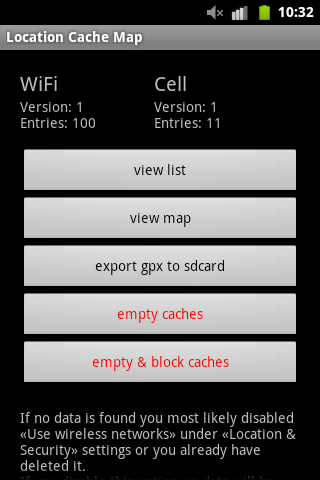
\includegraphics[width=5cm]{images/cache1.png}
  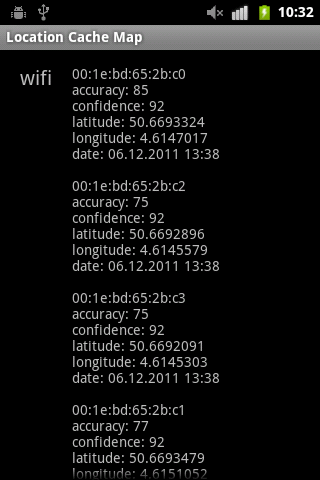
\includegraphics[width=5cm]{images/cache2.png}
  \caption{Captures from the application Location Cache by Remy Demy}
  \label{fig:locmap}
\end{figure}

The recent criticism about privacy concerns is mainly based on the existence of these cache files.
If the iOS devices used to have unlimited cache size (fixed in iOS 4.3.3), on an Android device, only the 50 last cells and 200 access points have been observed as stored in the cache files.
% TODO add reference prev sentence
However, in the course of this research, the observations made based on the analysis of the data collected from several devices have shown that this size is enough to contain locations older than one month.
A forensic analysis would allow to retrieve the device location at a given time if a location request was made.
Such requests can be run in background by any application having the correct permissions.
The DroidWatcher application relays on this fact to monitor the location of the user in background.\\

To show the ease of retrieving such information, a python script has been developed~\cite{soft-locdump} to parse the content of these two files and produce a GPS trace file in GPX format\footnote{GPX is a XML file format listing geographical coordinates with timestamp and allowing to reproduce the movement of a device} representing the approximate movement of the device.
However, a root access to the phone is required to access these files\footnote{Most of the time, granting a root access requires a system manipulation and voids the manufacturer warranty.}.
This could prevent malicious applications retrieving these data.
This cache folder is only created when the \emph{Use wireless networks} option is enabled in the Android settings.
However, this option is often required by common applications such as Google Maps which may lead to a large percentage of devices having this option enabled.\\

\section{Cell tower}
\label{sec:loc-cell-tower}
Similar to the method used with wireless access points, a cell tower can be identified in a unique way.
A GSM cell tower is characterised by two factors: a Location Area Code regrouping tens or hundreds of cell towers and a Cell ID identifying a cell tower inside a location area.
It is the combination of these two factors that enables a device to identify a unique cell tower.
A cellphone can then be located using trilateration based on the surrounding cell towers.\\

The data collection method and cache management system are very similar to the ones analysed in Section \ref{sec:andro-wifi} and will not be discussed here.
The location system in Android use usually both wireless access points and cell towers location methods simultaneously and indifferently for the user and developer.
The advantage of using cell tower location over the wireless is the fact it allows to locate a device with an approximate accuracy of 1km almost everywhere.

%In the DroidWatcher application (see Chapter \ref{chap:droidwatcher}), the application implements its own trilateration algorithm for offline computation.

\section{Privacy concerns}
\label{sec:andro-priv}

\subsection{Google Cars}
In May 2010, Google admitted to German authorities having collected more than what it was supposed to.
In addition to access point's unique identifier, it had ``been mistakenly collecting samples of payload data from open networks''.
These data chunks could include parts of web surf, email, text...\footnote{TechEYE, May 2012, \url{http://news.techeye.net/security/google-admits-it-sniffed-out-peoples-data}}.
In reaction, the data collected was asked to be deleted and the CNIL (independent French administrative authority) fined Google with €100.000\footnote{BBC UK, Mar 2011, http://www.bbc.co.uk/news/technology-12809076}.\\

\subsection{\_nomap}

Some users considered the collected data by the Google Cars and Android devices as private.
In November 2011, in reaction to criticism, Google created a way to opt out recording of its access point.
The proposition of Google is to end the ESSID of the wireless access point with \texttt{\_nomap}.
The next time it is scanned by a Google Cars or an Android device, the access point is removed from the database.
Google hopes than over time, the \texttt{\_nomap} string will be adopted by other location providers~\cite{nomap}.\\

This proposition was received with much of scepticism and did not satisfy the pro-privacy groups.
The main complain was the need of an action from the user to explicitly opt out its access point while people wants a way to explicitly opt in instead.
Many people that are concerned by privacy issues do not have enough technical knowledge to modify the wireless network name.
Furthermore, if this string is not universally adopted by other companies such as Apple or SkyHook, conflicting systems can be imagined, preventing a concerned user to fully opt out its access points from commercial databases.

\subsection{Research of Samy Kamkar}
\label{sec:andro-samy}

To reply to privacy concerns, Google ensured ``The location information sent to Google servers when users opt in to location services on Android is anonymised and stored in the aggregate and is not tied or traceable to a specific user''~\cite{loc-not-traceable}.
The security researcher Samy Kamkar has also looked at the location requested.\\

% \begin{figure}[h]
%   \hspace*{-2cm}
%   \centering
%   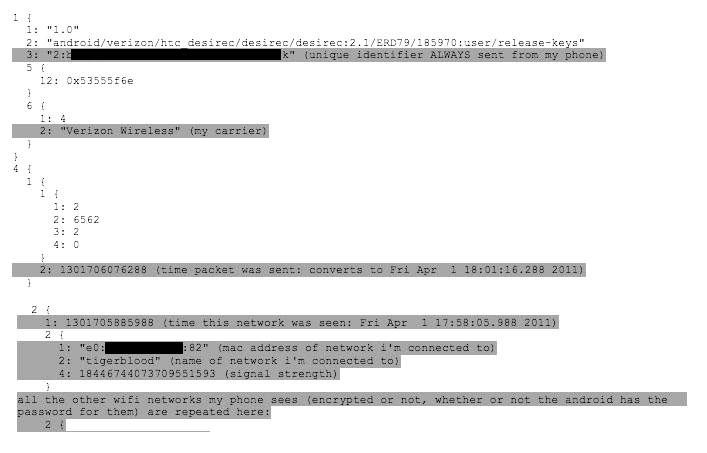
\includegraphics[width=18cm]{images/reqdecode.jpg}
%   \caption{Decrypted request content reveal to CNet by Samy Kamkar}
%   \label{fig:reqdecode}
% \end{figure}

He succeeded to decrypt the request made to Google servers and realised that it contains a unique identifier~\cite{cnet-andr-samy}.
%Figure \ref{fig:reqdecode} is the content of a request decrypted by Samy Kamkar sent to CNet.
% TODO rewrite the graph ?
The identifier is unique to the cell phone and present in every request.
If this string does not directly reveal the identity of the phone owner, it is however possible to tied the string to a specific user and then trace him.
He affirms there is no proof the location is anonymised due to the presence of this identifier.\\

\section{Personal researches}
\label{sec:andro-perso-research}

Several facts about the storage of information and privacy have been announced.
% TODO ajouter source
To verify these facts, further investigations have been carried in this thesis.
The applications used to realise the analyses are presented in the appendix.\\
% TODO mettre numero de appendix

To realise the experiments a rooted smartphone using Android 2.3 was used.
As most of the location information, including the cache databases files, are located in restricted part of the system, the rooting was necessary to explore the whole content of the phone.
The root process and implications are discussed in the introduction.

\subsection{Experiment 1: Database suppression}

\subsubsection{Goal}

When the option \emph{Use wireless networks} in the system settings is disabled, Google ensured the cache files are deleted.
The cache files have been located long ago but the question is to know if it was the only place that stored this location information.\\

During this experiment, the content of the device is inspected before and after opting out the option \emph{Use wireless networks} and the two versions are compared to detect the modified or deleted files.

\subsubsection{Methodology}

\begin{enumerate}
\item Make a dump of the internal memory
\item Disable the \emph{Use wireless networks} option
\item Make a dump of the internal memory
\item Compare the two dumps
\end{enumerate}

To facilitate the experiment realisation the two scripts \texttt{androdump.py} and \texttt{compare\_dump.py} have been developed and are available on the appendix %TODO the CD-ROM or url
The dump is done using the script \texttt{androdump.py} which uses the Android Debug Bridge (adb) program connecting the device to a computer.
The comparison is done using the script \texttt{compare\_dump.py} which uses a hash function on each file present in the dump to detect a modification.

\subsubsection{Result}

The goal of the comparison was to ensure that only the folder containing the databases is altered and the information is not stored somewhere else.
The analysis reveals that, with the exception of some irrelevant system files (battery state...) modified, the database files only are updated.
The cache data of Google Maps application has been also deleted.
This confirms the assumption concerning the deletion of location data.\\

\subsection{Experiment 2: Impact of location requests}

\subsubsection{Goal}

When a location is requested on an Android device, the system sends an encrypted request to Google's location servers.
Google's servers reply to the request with the location of surrounding GSM cell towers and access points.\\

The goal of the experiment was to detect the impact of a location request.
It is known that the surrounding wireless access points and cell towers information is stored in the cache file but other location related information could be stored somewhere else.
This experiment inspects the content of the system before and after a localisation request is made.

% To understand the content of the requests, two analyses have been made.
% The first one aimed to ensure the location informations are stored only in the two cache folders.
% The second one is an analysis of the volume of transmitted data correlated to the number of entries added in cache.\\

\subsubsection{Methodology}

\begin{enumerate}
\item Make a dump of the internal memory
\item Request the current location
\item Make a dump of the internal memory
\item Compare the two dumps
\end{enumerate}

The Android application \texttt{LocateMe} has been developed to create a simple location request using the network provider (including GSM cell towers and wifi access points).
% TODO preparer réponse si poste des questions sur les irrelevant system files

\subsubsection{Result}

The analysis reveals that, with the exception of irrelevant system files, only the database cache files have been modified.\\

\subsection{Experiment 3: Correlation between size and cache of requests}

\subsubsection{Goal}

As the request used to locate the device using wifi and cell towers is encrypted, its content is unknown.
What is known and confirmed in the previous experiments is the fact that the cache files are updated and some wifi and cell towers information are added to these files when a request is made.
To guess the content of a location request, it has been tried to determine patterns in the requests form to correlate a request with the content of the cache files.

\subsubsection{Methodology}

\begin{enumerate}
\item Start in \emph{blank state}\footnote{\emph{Blank state} : wireless turned off, empty location cache, location permission turned off, no process requiring the location such as Google Maps running.}
\item Start monitoring the traffic
\item Activate the wireless
\item Request the current location
\item Stop monitoring the traffic once a location received
\end{enumerate}

The network monitoring has been made with the tool \emph{tcpdump}\footnote{TCPDUMP 4.3 \url{http://www.tcpdump.org/}} installed on the Android device.

\begin{figure}[h]
  \centering
  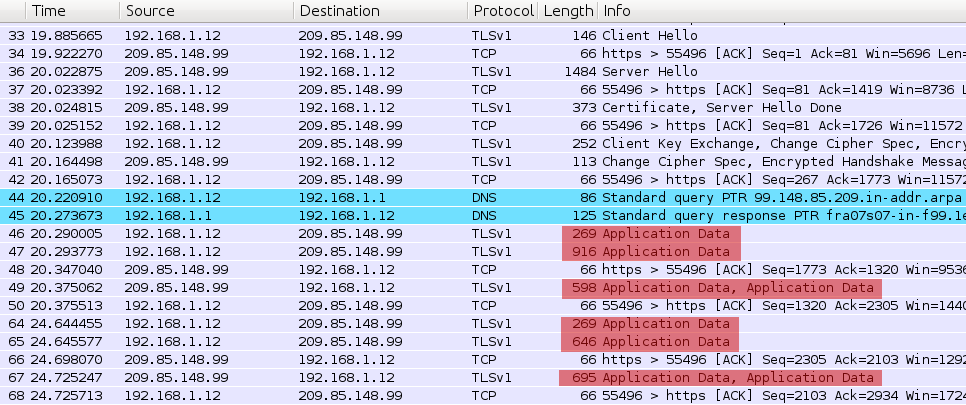
\includegraphics[width=\textwidth]{images/trace2.png}
  \caption{Example of tcpdump capture while a location request displayed in Wireshark}
  \label{fig:loc-req-tcpdump}
\end{figure}

\subsubsection{Result}

From the collected trace, the size of the transmitted data was compared with the number of cells and access points added to the cache files.
After observation and repeating the experiment (results displayed in Table \ref{tab:expe-req-pattern}), the following observations were made.
Each location requests is composed of two communications with Google's servers.
In each communication, a first packet of 271 bytes is sends followed by another of variable size.\\

% \begin{itemize}
% \item Two requests are made, one for the cells, one for the wifi.
% \item The first packets contains every time 269 bytes.
% \item The uploaded data size is larger than the downloaded.
% \item The size of the downloaded data is directly linked to the number of entries in the cache files.
% \end{itemize}

\begin{table}[h]
  \centering
  \begin{tabular}[h]{ |l|l|l|l|l|l|}
    \hline
    S. cell & S. wifi & Req 1 & Req 2 & C. cell & C. wifi \\
    \hline
    6 (1)    &     4 & 271+644/654 & 271+879/817 & 2 (1) & 4 \\
%    \hline
%    7 (1)    &     5 & 271+644/655 & 271+879/817 & 2 (1) & 5 \\
    \hline
    1       &   3  & 271+428/619 & 271+576/713 & 1 & 3 \\
    \hline
    4 (1) & 9 & 271+463/632 & 271+898/861 & 2 (1) & 9 \\
    \hline
    6 (1) & 10 & 271+434/619 & 271+916/873 & 1 & 10 \\
    \hline
  \end{tabular}
  \caption{Example of location requests and effect on the cache files}
  \label{tab:expe-req-pattern}
\end{table}

Table \ref{tab:expe-req-pattern} shows data collected during the experiments realised.
\textbf{S. cell} represents the number of surrounding valid GSM cell towers at the collect time.
$6 (1)$ means there is six surround GSM cell towers detected but only one is valid\footnote{Some cell towers are detected but displayed as using a Cell ID and LAC of -1, these are considered as invalid and ignored. These invalid cells have often a very weak signal strength.}.
\textbf{S. wifi} represents the number of surrounding wireless access points at the collect time.
\textbf{Req 1} represents the first communication and \textbf{Req 2} the second ($271+644/654$ means two packets of 271 and 644 bytes are uploaded and 654 bytes are downloaded from Google's servers).
\textbf{C. cell} represents the number of cell towers and \textbf{C. wifi} the number of wireless access points in the cache files after the location request (numbers between parenthesis represents the number of valid entries in the cache file, as the experiment starts in blank state, the cache files are empty at start).\\


Figure \ref{fig:loc-req-tcpdump} shows an example of collected trace confirming the derived pattern.
The packets number 46 and 64 contain 269 bytes and are the initiating packets of a request for cell towers and wireless access points.
The packets number 47 and 65 are the surrounding cell towers and access points uploaded to Google servers.
The packets number 49 and 67 are the reply from Google's servers containing the coordinates of the known cell towers and access points.
These observations do not allow to validate the suppositions concerning the content of the packet but the patterns are coherent to the model explained before.

\subsection{Experiment 4: Unique identifier}

\subsubsection{Goal}

As mentioned in Section \ref{sec:andro-samy}, Samy Kamkar observed that an unique identifier was used in the requests made to Google servers.
The presence of this identifier could compromise the privacy of the user as it would allow Google to trace a location requests to a certain user.
The purpose of this experiment was to verify this fact.

\subsubsection{Methodology}

Personal examinations of the cache folder in the system file showed that this string is contained inside a file \texttt{gls.platform.key} next to the cache database.
When the option \emph{Use wireless networks} in the Android settings is disabled, the content of the cache location folder (containing the wifi and cell cache files as well as this identifier) is emptied.
When the option is enabled, new cache files and unique identifier are create.
The content of the identifier file \texttt{gls.platform.key} is different to the previous value every time the option is toggled.
%\texttt{/data/data/com.google.android.location/files/gls.platform.key} 

\subsubsection{Conclusions}

The traceability possibility are limited due to this constrain.
If it is relatively easy to change this value, we can however imagine that very few users are aware of the existence of this value and will apply this manipulation regularly.


% \subsection{Android API}
% When an application wants to locate the device position, the Android system provides some higher level methods to use the available technologies listed above. Getting a user location in Android works by means of callback. A \texttt{LocationListener} is defined and will react to event such as \texttt{onLocationChanged} or \texttt{onProviderEnabled}. On the relevent event, the callback function is executed and the location retrieved~\cite{doc-location}.

% \lstset{language=Java}
% \begin{lstlisting}[label=location-base,caption=Code from Android developers guide]
% // Acquire a reference to the system Location Manager
% LocationManager locationManager = (LocationManager) this.getSystemService(Context.LOCATION_SERVICE);

% // Define a listener that responds to location updates
% LocationListener locationListener = new LocationListener() {
%     public void onLocationChanged(Location location) {
%       // Called when a new location is found by the network location provider.
%       makeUseOfNewLocation(location);
%     }

%     public void onStatusChanged(String provider, int status, Bundle extras) {}

%     public void onProviderEnabled(String provider) {}

%     public void onProviderDisabled(String provider) {}
%   };

% // Register the listener with the Location Manager to receive location updates
% locationManager.requestLocationUpdates(LocationManager.NETWORK_PROVIDER, 0, 0, locationListener);
% \end{lstlisting}
  
% At any moment, a user can request the last known location using the following code

% \begin{lstlisting}[label=getLastKnown,caption=Get the last recorded location]
% LocationProvider locationProvider = LocationManager.NETWORK_PROVIDER;
% // Or use LocationManager.GPS_PROVIDER

% Location lastKnownLocation = locationManager.getLastKnownLocation(locationProvider);
% \end{lstlisting}

% The provider \texttt{GPS\_PROVIDER}  or \texttt{NETWORK\_PROVIDER} allows to choose the source of the location. The GPS is used in the first case and an hybrid method using both wireless and cell tower location in the second.\\

% A \texttt{Location} is characterized by the following parameter that can be used to determined if a location is or not relevant by an application :
% \begin{itemize}
% \item Logitude
% \item Latitude
% \item Altitude
% \item Provider (GPS, Network...)
% \item Accuracy
% \item Time of the fix
% \end{itemize}
